\documentclass[11pt,a4paper]{article}

\usepackage[utf8]{vietnam}
\usepackage[margin=2.05cm]{geometry}
\usepackage{microtype}
\usepackage{setspace}
\usepackage{amsmath,amssymb}
\usepackage{graphicx}
\usepackage{booktabs}
\usepackage{tabularx}
\usepackage{array}
\usepackage{float}
\usepackage{xcolor}
\usepackage{enumitem}
\usepackage[numbers,sort&compress]{natbib}
\usepackage{hyperref}
\usepackage{xurl}

\hypersetup{
  colorlinks=true,
  linkcolor=blue!45!black,
  citecolor=blue!45!black,
  urlcolor=blue!55!black,
  pdftitle={Báo cáo tái lập Null-TTA, DAS và Feynman--Kac steering}
}
\setstretch{1.07}
\setlength{\parindent}{0pt}
\setlength{\parskip}{0.52em}
\setlist{nosep,leftmargin=1.5em}
\newcolumntype{Y}{>{\raggedright\arraybackslash}X}
\newcommand{\code}[1]{\texttt{#1}}
\newcommand{\PASS}{\textcolor{green!42!black}{\textbf{PASS}}}
\newcommand{\FAIL}{\textcolor{red!72!black}{\textbf{FAIL}}}
\newcommand{\PARTIAL}{\textcolor{orange!82!black}{\textbf{PARTIAL}}}
\newcommand{\PWV}{\textcolor{blue!60!black}{\textbf{PASS WITH VARIANCE}}}
\newcommand{\NullVerdict}{PASS}
\newcommand{\NullPickMean}{0.316}
\newcommand{\NullPickSD}{0.001}
\newcommand{\NullPickCILow}{0.308}
\newcommand{\NullPickCIHigh}{0.324}
\newcommand{\NullPickSymDiff}{0.2\%}
\newcommand{\NullPickImprovement}{0.097}
\newcommand{\NullPickImprovementCILow}{0.089}
\newcommand{\NullPickImprovementCIHigh}{0.106}
\newcommand{\DASVerdict}{PASS\_WITH\_VARIANCE}
\newcommand{\DASCanonicalEMD}{0.743}
\newcommand{\DASCanonicalSymDiff}{9.8\%}
\newcommand{\DASThreeMean}{1.025}
\newcommand{\DASThreeSD}{0.704}
\newcommand{\DASWorstSeed}{43}
\newcommand{\DASWorstEMD}{1.826}
\newcommand{\KaggleEMD}{1.496}
\newcommand{\KaggleReward}{-3.230}
\newcommand{\KagglePaperSymDiff}{58.4\%}
\newcommand{\KaggleModalSymDiff}{67.2\%}
\newcommand{\KagglePaperVerdict}{FAIL}
\newcommand{\KaggleModalVerdict}{FAIL}
\newcommand{\FKCVerdict}{PASS\_WITH\_VARIANCE}
\newcommand{\FKCWithinOneSD}{24}
\newcommand{\FKCWithinTwoSD}{30}
\newcommand{\FKCDirectionAgreement}{19}
\newcommand{\FKCElapsedMinutes}{17.4}
\newcommand{\FKCCost}{0.367}
\newcommand{\FKCMaxVRAM}{7.99}
\newcommand{\BillingTungSixUsage}{27.68}
\newcommand{\BillingTungSixCost}{21.41}
\newcommand{\BillingTungSixHeadroom}{1.32}
\newcommand{\BillingTungEightUsage}{25.05}
\newcommand{\BillingTungEightCost}{20.42}
\newcommand{\BillingTungEightHeadroom}{3.95}
\newcommand{\BillingVuHoanUsage}{27.29}
\newcommand{\BillingVuHoanCost}{25.07}
\newcommand{\BillingVuHoanHeadroom}{1.71}


\title{\textbf{Báo cáo tái lập thực nghiệm có kiểm toán}\vspace{0.2em}\\
\large Null-TTA, DAS, FK Steering và Feynman--Kac Correctors}
\author{Báo cáo kỹ thuật từ artifact remote, multi-seed và provenance khóa phiên bản}
\date{12 tháng 8 năm 2026}

\begin{document}
\maketitle

\begin{abstract}
Báo cáo này tái lập Table~1 SD-v1.5 của Null-TTA (CVPR 2026), Figure~1 GMM của DAS và toàn bộ sáu hàng Table~A1 GMM của Feynman--Kac Correctors; đồng thời giữ lại thí nghiệm một prompt của FK Steering để tạo một hồ sơ thống nhất. Null-TTA được đánh giá trên đủ 50 prompt chính thức, ba seed và bốn scorer thật. DAS được chạy lại sau khi phát hiện RNG của Numba độc lập với NumPy: seed Python/Torch và Numba được khóa trùng nhau, EMD được báo theo cả estimator một lần giống notebook paper và 100 lần lặp để đo độ bất ổn. FK Correctors dùng đúng 10,000 samples, 1000 integration steps và 5 sequential stochastic runs cho no-FKC, birth--death clocks và systematic resampling. Một bản DAS seed~42 cũng được triển khai trên Kaggle T4x2. Mọi thí nghiệm khoa học chạy remote trong môi trường \code{uv --frozen}; máy local chỉ điều phối, tổng hợp, vẽ hình và biên dịch tài liệu. Báo cáo tách rõ ba câu hỏi: code có chạy không, point estimate có tái lập không, và kết quả có ổn định qua seed/run không.
\end{abstract}

\textbf{Từ khóa:} test-time alignment, diffusion, Null-TTA, Sequential Monte Carlo, Feynman--Kac, reproducibility.

\section{Kết luận điều hành}

\begin{table}[H]
\centering
\small
\caption{Verdict chỉ áp dụng cho phạm vi đã chạy, không được ngoại suy thành benchmark-wide superiority.}
\begin{tabularx}{\textwidth}{@{}p{2.45cm}p{3.35cm}Yp{2.45cm}@{}}
\toprule
Công trình & Phạm vi & Kết luận có thể bảo vệ & Verdict \\
\midrule
Null-TTA & Table 1 SD-v1.5, 50 prompt, seed 42--44, target PickScore & Primary PickScore đạt \NullPickMean{} (paper 0.315), bootstrap CI $[\NullPickCILow,\NullPickCIHigh]$, sai khác đối xứng \NullPickSymDiff. & \textbf{\NullVerdict} \\
DAS & Figure 1 GMM, official SMC, matched Numba RNG & Seed mặc định 42 đạt EMD \DASCanonicalEMD{} so với paper 0.82; ba seed vẫn có variance rất lớn. & \PWV \\
DAS Kaggle & Seed 42, allocation T4x2, workload chính thức dùng một GPU & Hạ tầng và payload khoa học hoàn chỉnh; numeric portability được chấm riêng với paper và Modal. & xem Sec.~\ref{sec:kaggle} \\
FK Steering & Một prompt, ba seed, $k=4$, ImageReward & Pipeline chạy được nhưng variance lớn và không đại diện GenEval. & \PARTIAL \\
FK Correctors & Exact Table A1: 10k samples, 1000 steps, 5 runs, 6 methods & \FKCWithinTwoSD/30 ô mean nằm trong paper mean $\pm2$ SD; variance FKC lớn và phải báo theo run. & \PWV \\
\bottomrule
\end{tabularx}
\end{table}

Hai ranh giới quyết định:
\begin{enumerate}
  \item \textbf{Không đổi tên reproduction thành improvement.} Null-TTA được chấm bằng độ gần point estimate Table~1 và cải thiện paired so với baseline cùng seed. DAS được chấm bằng EMD/mode fidelity trước reward; reward $-0.21$ không tự động tốt hơn $-0.22$ nếu target là $-0.29$.
  \item \textbf{Không dùng CI rộng để ``cứu'' một point estimate.} Với DAS, khoảng $t$ từ ba seed quá rộng và thậm chí có cận âm dù EMD không âm. Báo cáo dùng seed~42---seed mặc định công khai của notebook---cho exact-point reproduction, rồi báo ba seed như sensitivity analysis độc lập.
\end{enumerate}

\section{Hợp đồng đánh giá, từ điển metric và nguồn bằng chứng}

\subsection{Null-TTA: bốn scorer không cùng một đơn vị}

Null-TTA tối ưu embedding null-text $\varnothing_t$ ở inference time trong khi giữ nguyên trọng số diffusion. Với reward mục tiêu $R$, regularizer embedding và prior-preservation, dạng loss thực thi có thể tóm tắt là
\begin{equation}
\mathcal{L}_t = -\lambda_{\alpha}R(x_t,c)
 + \lambda_{\mathrm{reg}}\lVert\varnothing_t-\varnothing_t^{(0)}\rVert_2^2
 + \mathcal{L}_{\mathrm{prior}}.
\end{equation}
Paper báo Table~1 SD-v1.5 trung bình qua ba random seed nhưng không công bố ID seed. Protocol này dùng $\{42,43,44\}$ vì 42 là default trong code; đây là giả định minh bạch, không phải fact từ paper. Bốn cột của Table~1 đều là learned scorer nhưng đo các khía cạnh khác nhau; số tuyệt đối giữa hai scorer \emph{không} cùng đơn vị và không được so trực tiếp \citep{Kim2026NullTTA,NullTTACode}.

\begin{description}
  \item[PickScore $\uparrow$ (target metric).] Code dùng checkpoint \code{yuvalkirstain/PickScore\_v1}. Với ảnh $x$ và prompt $c$, image/text embedding được chuẩn hóa rồi lấy cosine theo đúng cặp:
  \begin{equation}
    S_{\mathrm{Pick}}(x,c)=
    \left\langle \frac{f_I(x)}{\lVert f_I(x)\rVert_2},
    \frac{f_T(c)}{\lVert f_T(c)\rVert_2}\right\rangle .
  \end{equation}
  Implementation reproduction không nhân logit scale và không softmax, nên giá trị là cosine (về toán học trong $[-1,1]$), \emph{không phải} xác suất người dùng chọn ảnh. Higher-is-better. Đây là reward được Null-TTA tối ưu trực tiếp; vì vậy nó là primary metric nhưng cũng là metric dễ chịu reward over-optimization nhất.

  \item[HPS v2 $\uparrow$ (held-out/cross-reward).] Scorer dùng HPSv2 ViT-H/14; image/text feature cũng được chuẩn hóa và lấy cosine của cặp tương ứng. Vì là một preference model khác PickScore, HPS v2 kiểm tra liệu gain có chuyển sang một proxy preference khác hay chỉ ``học mẹo'' của PickScore. Nó cũng không phải xác suất, và 0.29 HPS không thể so độ lớn trực tiếp với 0.29 PickScore.

  \item[Aesthetic $\uparrow$ (image-only).] Ảnh được mã hóa bằng CLIP ViT-L/14, feature được chuẩn hóa rồi đi qua MLP checkpoint \code{sac+logos+ava1-l14-linearMSE.pth}. Scorer không nhận prompt:
  \begin{equation}
    S_{\mathrm{aes}}(x)=g\!\left(f_I(x)/\lVert f_I(x)\rVert_2\right).
  \end{equation}
  Vì vậy nó đo proxy về vẻ đẹp/chất lượng thị giác, không đo prompt adherence. Giá trị quanh 5 trong bảng là output thô của regressor, không phải thang xác suất hay ``5 trên 10'' đã được calibration cho mọi domain.

  \item[ImageReward $\uparrow$ (held-out/cross-reward).] Scorer quantize tensor ảnh về uint8, dùng BLIP visual encoder, cho text encoder cross-attend vào image embedding, rồi MLP trả một scalar $S_{\mathrm{IR}}(x,c)$. Score có thể âm và không bị chặn ở $[0,1]$; nó là reward-model logit/utility thô, không phải xác suất. Higher-is-better. Do kiến trúc và dữ liệu học khác PickScore, đây là kiểm tra cross-reward mạnh hơn Aesthetic cho prompt--image alignment, nhưng vẫn chỉ là một learned proxy.
\end{description}

\textbf{Cách đọc đúng:} PickScore trả lời ``có tái lập đúng target paper không?''; ba scorer còn lại trả lời ``gain có generalize sang proxy khác không?''. Chúng giảm rủi ro reward hacking nhưng không thay thế human evaluation và không chứng minh universal preference. Primary estimand là optimized PickScore tại $n_{\max}=55$ so với point 0.315. PASS yêu cầu đồng thời symmetric relative difference
\begin{equation}
d_{\mathrm{sym}}(a,b)=\frac{|a-b|}{(|a|+|b|)/2}
\end{equation}
không quá 10\%, và CI 95\% bootstrap phân cấp của paired improvement so với chính baseline phải hoàn toàn dương. HPS~v2, Aesthetic và ImageReward là secondary numeric checks, không được dùng để thay primary sau khi xem kết quả. Mỗi paired improvement là $S(x_{\mathrm{Null}})-S(x_{\mathrm{base}})$ trên cùng prompt và seed; cách ghép cặp này loại bớt độ khó prompt khỏi sai số.

\subsection{DAS: reward không phải distributional fidelity}

DAS định nghĩa phân phối alignment
\begin{equation}
p_{\mathrm{tar}}(x) \propto p_{\mathrm{pre}}(x)\exp(r(x)/\alpha),
\end{equation}
tương đương tối ưu reward có KL regularization. Trong GMM notebook, $\alpha=1$ và
\begin{equation}
  r(x_1,x_2)=-\frac{x_1^2}{100}-x_2^2.
\end{equation}
Reward càng cao nghĩa là càng ít âm; trục $x_2$ bị phạt mạnh hơn $x_1$. Tuy nhiên target là \emph{toàn bộ} $p_{\mathrm{tar}}$, không phải điểm cực đại của $r$. Vì vậy score $-0.21$ không tự động ``tốt hơn'' paper $-0.22$ hoặc target $-0.29$: nó có thể báo mẫu bị kéo quá mạnh vào vùng reward cao và sai khối lượng mode.

Metric fidelity chính là multivariate Earth Mover's Distance, ở đây chính là empirical 1-Wasserstein với ground cost Euclidean:
\begin{equation}
  \widehat W_1(X,Y)=\min_{\pi\in\Pi(u_X,u_Y)}
  \sum_{i,j}\pi_{ij}\lVert x_i-y_j\rVert_2.
\end{equation}
Lower-is-better; 0 chỉ đạt khi hai empirical measure trùng nhau. \textbf{Paper-style EMD} là đúng một lần rút có hoàn lại 500 SMC và 500 target samples như notebook chính thức. \textbf{Stable EMD} là mean $\pm$ sample SD của 100 lần rút 500-vs-500 bằng RNG riêng cố định; nó đo noise của estimator, là diagnostic bổ sung của report chứ không phải metric mới của paper \citep{Kim2025DAS,DASCode}.

Mode diagnostics gán mỗi sample vào tâm GMM gần nhất. Một target mode là active nếu có ít nhất 1\% target mass; coverage đếm bao nhiêu active target mode cũng nhận ít nhất 1\% sample mass. Coverage 3/3 càng cao càng tốt, nhưng rất thô: seed vẫn có thể đạt 3/3 trong khi phân bổ sai nặng. Vì vậy artifact còn lưu $L_1$ mass error $\sum_k|\hat p_k-\hat q_k|$ và spurious mass ngoài target modes, cả hai lower-is-better. Primary paper point ở Figure~1 là EMD 0.82, reward DAS $-0.22$ và target reward $-0.29$. Exact-point criterion của protocol là EMD seed~42 trong 10\% theo $d_{\mathrm{sym}}$, đồng thời mọi seed sensitivity phải cover 3/3 target modes. Mean/SD ba seed được báo đầy đủ nhưng không dùng CI rộng để tạo PASS.

\subsection{FK Steering: metric và cách aggregate}

Thí nghiệm đã chạy dùng đúng ImageReward nêu trên, nên higher-is-better nhưng score vẫn là scalar thô, không phải probability. Với method $m$, seed $s$ và $k=4$ particles, điểm trên hình là
\begin{equation}
  \bar R_{m,s}=\frac{1}{4}\sum_{j=1}^{4}S_{\mathrm{IR}}(x_{m,s,j},c).
\end{equation}
Report sau đó lấy mean của ba $\bar R_{m,s}$ và sample SD qua seed. Artifact cũng lưu mean best-of-4, nhưng không dùng best-of-4 làm central claim vì chọn cực đại trả lời một câu hỏi khác và dễ lạc quan hơn mean population. FK-max và FK-difference là \emph{hai potential/resampling rule}, không phải hai metric: code FK-max dùng weight tỉ lệ $\exp[\lambda\max(r_t,r_{\mathrm{stored}})]$, còn FK-difference dùng $\exp[\lambda(r_t-r_{\mathrm{stored}})]$ trước kiểm tra ESS/resampling \citep{Singhal2025FKSteering,FKSteeringCode}. Một prompt $\times$ ba seed chỉ kiểm tra pipeline và variance cục bộ; nó không tái lập metric GenEval hoặc benchmark-wide superiority của paper.

\subsection{Feynman--Kac Correctors: năm khoảng cách của Table A1}

Table~A1 so empirical samples $X$ với target test samples $Y$ trong toy GMM bằng năm metric lower-is-better \citep{Skreta2025FKC,FKCCode}:

\begin{description}
  \item[$W_1$ và $W_2$.] Code giải exact optimal transport giữa hai empirical measure có uniform mass. $W_1$ dùng cost $\lVert x-y\rVert_2$; $W_2$ dùng cost bình phương rồi lấy căn:
  \begin{equation}
    W_p(X,Y)=\left[\min_{\pi\in\Pi(u_X,u_Y)}
    \sum_{i,j}\pi_{ij}\lVert x_i-y_j\rVert_2^p\right]^{1/p},\quad p\in\{1,2\}.
  \end{equation}
  Chúng đo geometry đầy đủ trong không gian mẫu; outlier bị phạt mạnh hơn ở $W_2$.

  \item[MMD.] Notebook báo output của biased squared MMD với kernel là tổng của 10 RBF:
  \begin{equation}
    k(x,y)=\sum_{\sigma\in 10^{\mathrm{linspace}(-2,0,10)}}
    \exp\!\left(-\frac{\lVert x-y\rVert_2^2}{2\sigma^2}\right),
  \end{equation}
  rồi tính $\widehat{\mathrm{MMD}}^2=\overline{k(X,X)}+\overline{k(Y,Y)}-2\overline{k(X,Y)}$. Tên cột rút gọn là MMD, nhưng quantity code trả là estimator bình phương. Multi-bandwidth giúp thấy sai khác ở nhiều scale; trị số phụ thuộc kernel/bandwidth nên không so trực tiếp với $W_1/W_2$.

  \item[TV.] Đây là histogram approximation, không phải exact total variation của hai density liên tục. Target định nghĩa lưới $200\times200$; code chuẩn hóa histogram rồi tính
  \begin{equation}
    \widehat{\mathrm{TV}}_{200}=\frac{1}{2}\sum_b|\hat p_b-\hat q_b|.
  \end{equation}
  Giá trị nằm trong $[0,1]$, lower-is-better, nhưng nhạy với bin edges/range và số mẫu.

  \item[Energy-W2.] Tên cột của paper là Energy-W2, nhưng implementation gọi \code{pot.emd2\_1d} trên scalar energies với default squared-Euclidean cost và \emph{không lấy căn}:
  \begin{equation}
    D_{E}=\min_{\gamma\in\Pi(u_X,u_Y)}
    \sum_{i,j}\gamma_{ij}|E(x_i)-E(y_j)|^2=W_2^2(E_\#X,E_\#Y).
  \end{equation}
  Do đó report giữ nhãn paper nhưng diễn giải quantity là squared transport cost giữa hai energy distributions. Metric này có thể nhỏ dù geometry 2D còn sai, nếu hai tập có histogram năng lượng giống nhau.
\end{description}

Table~A1 báo mean $\pm$ sample SD $s=\sqrt{\sum_i(z_i-\bar z)^2/(5-1)}$ của năm run cho sáu phương pháp. Báo cáo này yêu cầu trước hết đúng toàn bộ protocol (10,000 samples, 1000 integration steps, $dt=0.001$, 5 runs và đủ sáu hàng). Với mỗi ô, ``compatible'' nghĩa là reproduction mean nằm trong paper mean $\pm2$ paper-reported SD. Đây là compatibility band, \emph{không phải} confidence interval và không được diễn giải là hai phân phối đồng nhất. Numeric PASS yêu cầu cả 30/30 ô compatible; bảng còn báo riêng số ô trong $\pm1$ SD, hướng thay đổi FKC so với no-FKC và từng run xấu để không dùng mean che variance.

\subsection{Identity và môi trường}

\begin{table}[H]
\centering
\small
\caption{Nguồn chính thức và commit khóa. Upstream clone được giữ sạch; runtime wrapper chỉ thêm seed/provenance/metric persistence.}
\begin{tabularx}{\textwidth}{@{}p{2.4cm}Yp{4.3cm}@{}}
\toprule
Paper & Code chính thức & Commit \\
\midrule
Null-TTA \citep{Kim2026NullTTA} & \url{https://github.com/kthone/null-tta} \citep{NullTTACode} & \nolinkurl{337bf73037e9f24e9f844974d3287384abb610bf} \\
DAS \citep{Kim2025DAS} & \url{https://github.com/krafton-ai/DAS} \citep{DASCode} & \nolinkurl{2f4b2239f29ee59f80359bdfa5ed747b6d855a1e} \\
FK Steering \citep{Singhal2025FKSteering} & \url{https://github.com/zacharyhorvitz/Fk-Diffusion-Steering} \citep{FKSteeringCode} & \nolinkurl{9413005dee1e79f80fb4561a4a7ac8eec704281b} \\
FK Correctors \citep{Skreta2025FKC} & \url{https://github.com/martaskrt/fkc-diffusion} \citep{FKCCode} & \nolinkurl{aa6f5ed4a0ebb91329d4cd5823cc7e77c5e196e6} \\
\bottomrule
\end{tabularx}
\end{table}

Các remote đều dựng môi trường bằng \code{uv sync --frozen --no-install-project}. Null-TTA dùng Python~3.10, Torch~2.3.1, Diffusers~0.32.2 và scorer official. Seed 42--43 chạy L40S với hyperparameter paper. Seed~44 dùng memory-reduced path: generation chỉ giữ PickScore resident, sau đó load tuần tự Aesthetic/HPS/ImageReward và chấm lại đúng cặp PNG mà code official đã lưu. Bảy artifact hoàn chỉnh chạy L4 24GB. App L4 [7,14) bị dừng vì billing guard nhưng đã commit đủ CSV và tám PNG lossless cho bốn prompt [7,11); prefix này được kiểm hash, chuyển sang workspace còn sống và post-score trên L40S. Ba prompt [11,14) được sinh và chấm mới trên L40S. Không có dữ liệu nào từ provider-disabled retry được đưa vào thống kê. Cách cứu này bảo toàn ảnh đã sinh nhưng tạo hardware/scoring-path confound được giữ trong threats to validity. DAS và FK Correctors dùng Python~3.10, Torch~2.4.0+cu121 trên Modal L4; Kaggle dùng cùng DAS lockfile trên allocation hai Tesla T4. Full FK Correctors đạt peak CUDA allocated \FKCMaxVRAM{} GiB, hoàn tất trong \FKCElapsedMinutes{} phút với provider cost \FKCCost{} USD.

\section{Null-TTA nmax=55 trên backbone SD-v1.5}

\subsection{Thiết kế}

Chúng tôi chạy đủ prompt list 50 mục trong example chính thức, seed $\{42,43,44\}$, target PickScore, $n_{\min}=5$, $n_{\max}=55$, $K=3$ particles, 100 diffusion steps, Adam learning rate 0.01, $\lambda_{\alpha}=100$, $\lambda_{\mathrm{reg}}=0.002$, $\phi=0.01$ và tampering coefficient 0.008. Aggregator từ chối build nếu thiếu bất kỳ cặp seed--prompt nào, có scorer mock/disabled, config drift hoặc commit drift. CI 95\% của optimized metric dùng bootstrap phân cấp: resample seed rồi resample prompt index, 10,000 repeat.

\textbf{Ánh xạ trực tiếp tới Table~1 gốc:} bảng dưới giữ phương pháp theo hàng như paper. Hàng SD-v1.5 tái lập \emph{hàng đầu tiên} (backbone chưa alignment); hàng Null-TTA $n_{\max}=55$ tái lập \emph{hàng cuối cùng} (cùng backbone sau tối ưu null-text embedding). Mỗi prompt--seed trong run chính thức sinh cả output baseline và output optimized; verdict Null-TTA được chấm trên output optimized, đồng thời giữ baseline làm paired control.

\subsection{Kết quả chính}

\begin{table}[H]
\centering
\small
\caption{Point estimate theo layout dễ đối chiếu với Table~1 gốc: phương pháp/nguồn theo hàng, bốn metric theo cột. Mũi tên chỉ hướng tốt hơn trong từng metric; không so độ lớn giữa các cột.}
\begin{tabular}{@{}lrrrr@{}}
\toprule
Nguồn / phương pháp & PickScore $\uparrow$ & HPS v2 $\uparrow$ & Aesthetic $\uparrow$ & ImageReward $\uparrow$ \\
\midrule
Paper / SD-v1.5 & 0.218 & 0.279 & 5.232 & 0.339 \\
Reproduction / SD-v1.5 & 0.218 & 0.279 & 5.230 & 0.337 \\
\addlinespace[2pt] Paper / Null-TTA $n_{\max}=55$ & 0.315 & 0.294 & 5.431 & 0.946 \\
Reproduction / Null-TTA $n_{\max}=55$ & 0.316 & 0.294 & 5.471 & 0.893 \\
\bottomrule

\end{tabular}
\end{table}

\begin{table}[H]
\centering
\footnotesize
\caption{Uncertainty và gate tái lập cho hàng Null-TTA. $\Delta$ là paired Null-TTA trừ SD-v1.5 trên cùng prompt--seed; CI 95\% dùng hierarchical bootstrap qua seed rồi prompt. Match chỉ chấm point estimate reproduction với hàng Null-TTA của paper bằng ngưỡng $d_{\mathrm{sym}}\leq10\%$.}
\begin{tabular}{@{}lrrrl@{}}
\toprule
Metric & Repro Null-TTA [CI 95\%] & Paired $\Delta$ [CI 95\%] & $d_{\mathrm{sym}}$ & Match \\
\midrule
PickScore & 0.316 [0.308, 0.324] & 0.097 [0.089, 0.106] & 0.2\% & \PASS \\
HPS v2 & 0.294 [0.289, 0.299] & 0.015 [0.012, 0.018] & 0.1\% & \PASS \\
Aesthetic & 5.471 [5.335, 5.603] & 0.240 [0.121, 0.355] & 0.7\% & \PASS \\
ImageReward & 0.893 [0.665, 1.111] & 0.556 [0.345, 0.756] & 5.8\% & \PASS \\
\bottomrule

\end{tabular}
\end{table}

\begin{table}[H]
\centering
\small
\caption{Sensitivity theo seed trên 50 prompt; không chọn riêng best seed. Các cột Null là output Null-TTA, Pick base là paired SD-v1.5 control.}
\begin{tabular}{@{}rrrrrr@{}}
\toprule
Seed & Pick base & Pick Null & HPS Null & Aesthetic Null & ImageReward Null \\
\midrule
42 & 0.219 & 0.314 & 0.294 & 5.531 & 0.862 \\
43 & 0.217 & 0.317 & 0.294 & 5.469 & 0.970 \\
44 & 0.219 & 0.316 & 0.294 & 5.412 & 0.846 \\
\bottomrule

\end{tabular}
\end{table}

\begin{figure}[H]
\centering
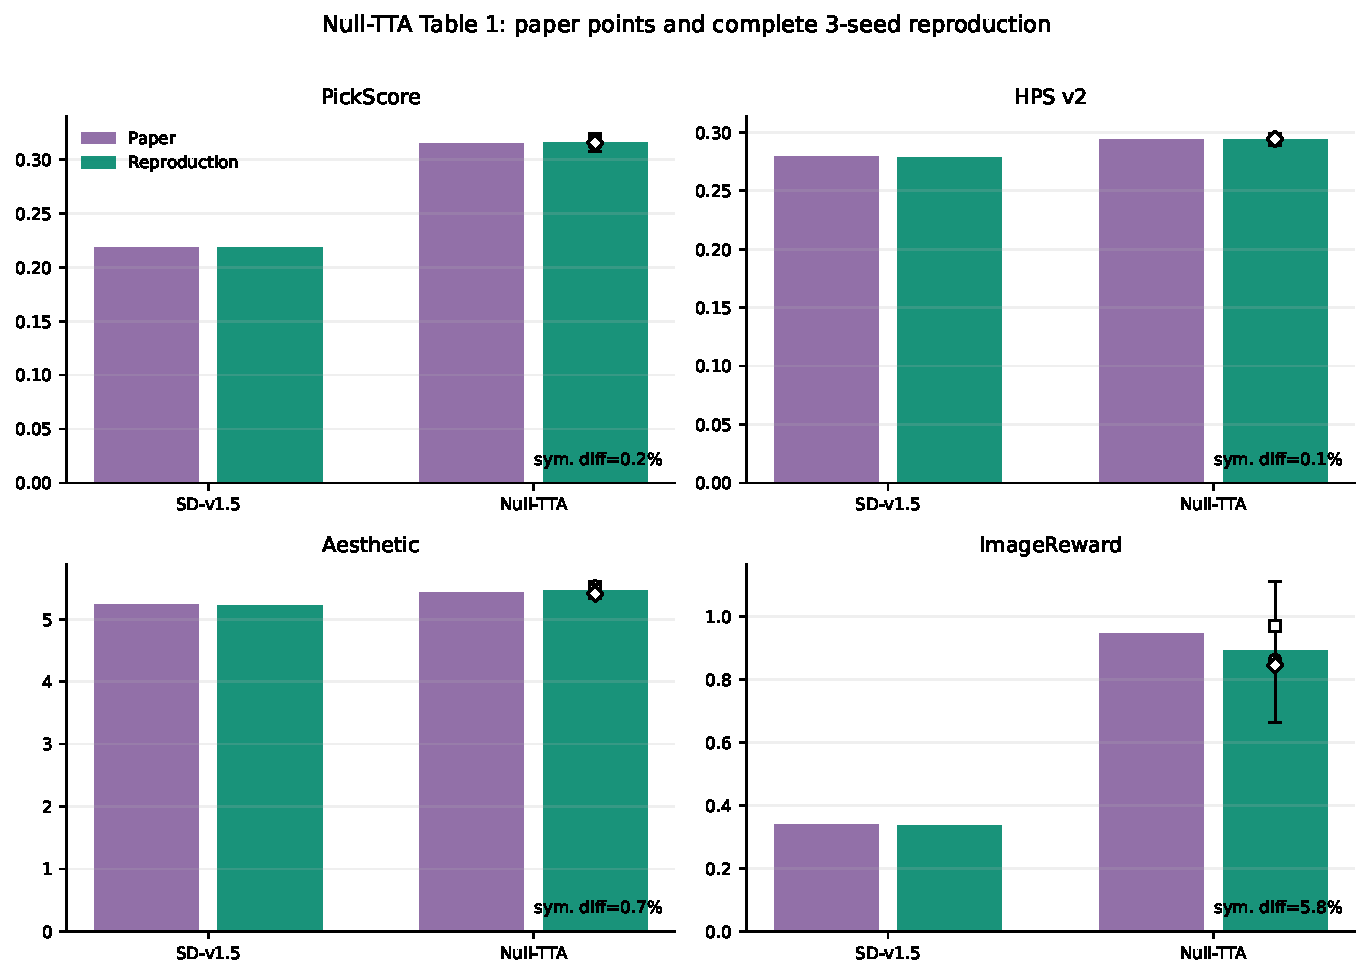
\includegraphics[width=0.96\textwidth]{figures/fig_null_tta_table1.pdf}
\caption{Bốn metric Table~1. Nhóm SD-v1.5 tương ứng hàng đầu tiên của bảng gốc; nhóm Null-TTA tương ứng hàng cuối cùng. Bar là paper/reproduction; marker trắng là từng seed; error bar của optimized reproduction là bootstrap CI 95\%. Mỗi panel dùng scale riêng, tránh chuẩn hóa che sai khác tuyệt đối.}
\label{fig:null-table}
\end{figure}

\begin{figure}[H]
\centering
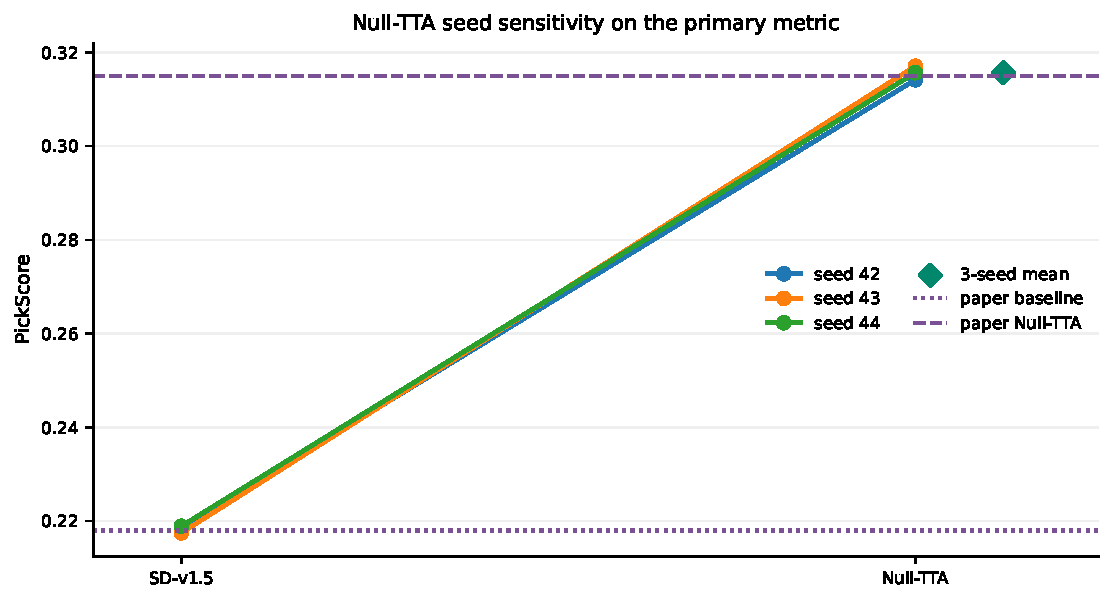
\includegraphics[width=0.82\textwidth]{figures/fig_null_tta_seed_variance.pdf}
\caption{Primary PickScore theo seed. Mỗi đường nối baseline và optimized trên cùng seed; đường ngang là point estimate paper.}
\label{fig:null-seed}
\end{figure}

Primary verdict machine-readable là \textbf{\NullVerdict}: PickScore reproduction \NullPickMean{}$\pm$\NullPickSD{} giữa seed, sai khác \NullPickSymDiff{} so với 0.315. Paired improvement là \NullPickImprovement{}, bootstrap CI 95\% $[\NullPickImprovementCILow,\NullPickImprovementCIHigh]$. Verdict này chỉ nói numeric reproduction của cấu hình Table~1; nó không chứng minh phương pháp mới tốt hơn Null-TTA hoặc vượt một prior work khác.

\section{DAS: matched-RNG rescue và variance}

\subsection{Vì sao kết quả cũ lệch}

Notebook chính thức seed Python, NumPy và Torch bằng 42, nhưng resampling kernel dùng Numba \code{@njit}; RNG của Numba có state riêng và không được seed bởi \code{np.random.seed} ở Python. Các run cũ vì vậy nhìn có vẻ ``cùng seed'' nhưng thực tế SMC resampling thay đổi không kiểm soát. Rescue thêm một hàm Numba-jitted gọi \code{np.random.seed(seed)} trước SMC, đồng thời đặt \code{CUBLAS\_WORKSPACE\_CONFIG=:4096:8}, tắt TF32 và bật deterministic algorithms trước khi CUDA khởi tạo.

\subsection{Kết quả}

\begin{table}[H]
\centering
\small
\caption{DAS theo matched Python/Torch/Numba seed. Paper-style EMD dùng đúng một subsample 500-vs-500; stable EMD là mean $\pm$ SD của 100 repeat.}
\begin{tabular}{@{}rrrrrr@{}}
\toprule
Seed & Paper-style EMD & Stable EMD & SMC reward & Modes & Diff. tới 0.82 \\
\midrule
42 & 0.743 & 0.546 $\pm$ 0.105 & -0.235 & 3/3 & 9.8\% \\
43 & 1.826 & 1.677 $\pm$ 0.174 & -0.268 & 3/3 & 76.0\% \\
44 & 0.505 & 0.441 $\pm$ 0.086 & -0.238 & 3/3 & 47.5\% \\
\bottomrule

\end{tabular}
\end{table}

Seed mặc định 42 đạt EMD \DASCanonicalEMD{}, cách paper 0.82 đúng \DASCanonicalSymDiff{} theo metric đối xứng: numeric reproduction PASS. Tuy nhiên, mean ba seed là \DASThreeMean{}$\pm$\DASThreeSD{}; mean này không đạt tolerance 10\%. Seed \DASWorstSeed{} là bad seed rõ rệt với EMD \DASWorstEMD{}. Vì vậy verdict đầy đủ là \textbf{\DASVerdict}: paper point được tái lập ở canonical seed nhưng claim không ổn định qua seed.

\begin{figure}[H]
\centering
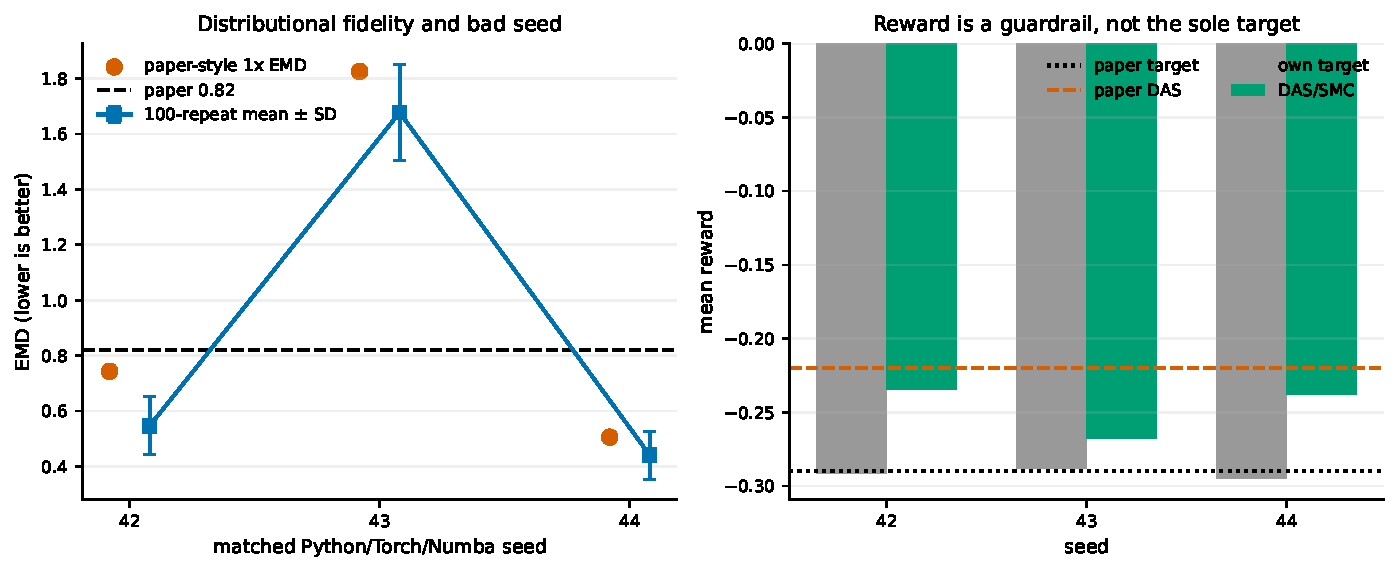
\includegraphics[width=\textwidth]{figures/fig_das_rescue_variance.pdf}
\caption{EMD/reward theo seed. Panel trái tách stochastic point estimator của paper khỏi mean 100 repeat; panel phải nhắc rằng reward phải đọc cùng target distribution.}
\label{fig:das-var}
\end{figure}

\begin{figure}[H]
\centering
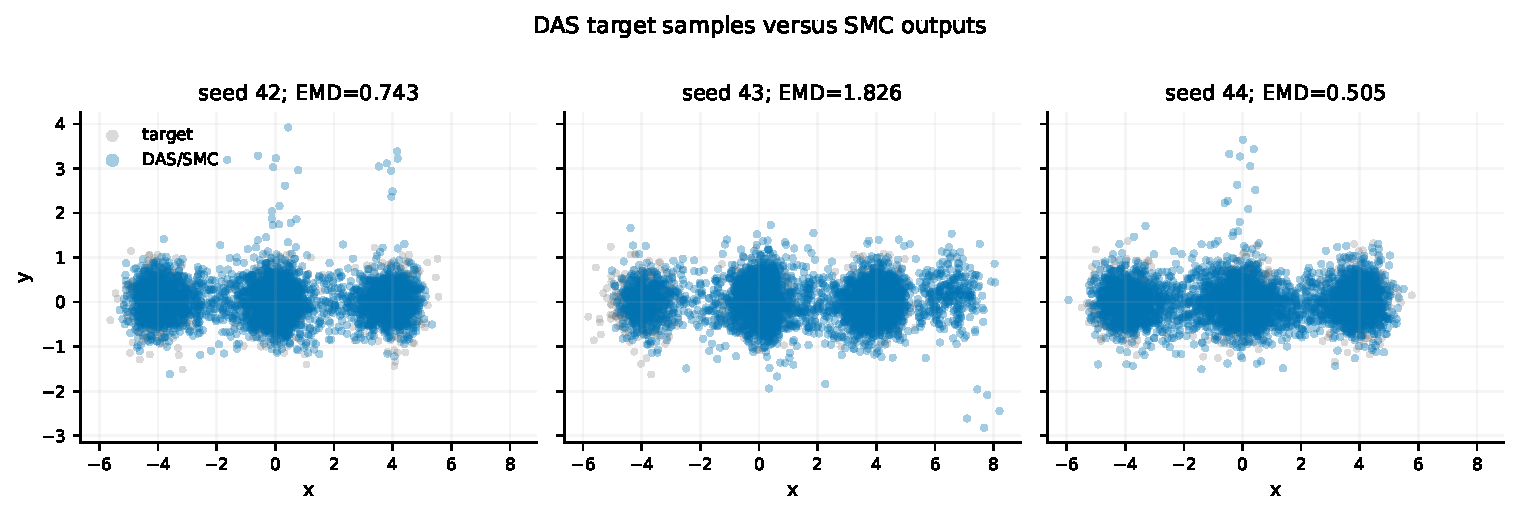
\includegraphics[width=\textwidth]{figures/fig_das_rescue_samples.pdf}
\caption{Target và SMC outputs đã lưu. Seed 43 vẫn cover ba mode theo threshold 1\% nhưng phân bổ mass sai nhiều, phù hợp EMD lớn.}
\label{fig:das-samples}
\end{figure}

\section{DAS trên Kaggle T4x2}\label{sec:kaggle}

Kernel chính thức là \url{https://www.kaggle.com/code/codemaivanngu/diffusion-smc-das-seed42-numba-rescue-t4x2-r6}. Accelerator probe xác nhận hai Tesla T4 visible; notebook DAS upstream vẫn chọn một device nên đây là portability run trên shape T4x2, không phải data-parallel speedup. Source package được embed thành archive deterministic có hash và bung vào \code{/kaggle/working/repo}; lockfile, upstream notebook và runtime patch giống Modal.

\begin{table}[H]
\centering
\small
\caption{Seed 42 trên paper, Modal và Kaggle. EMD là estimator một lần giống paper.}
\begin{tabular}{@{}lrrr@{}}
\toprule
Metric & Paper & Modal L4 & Kaggle T4x2 \\
\midrule
Paper-style EMD & 0.820 & \DASCanonicalEMD{} & \KaggleEMD{} \\
SMC reward & -0.220 & -0.235 & \KaggleReward{} \\
Target-mode coverage & -- & 3/3 & 3/3 \\
\bottomrule
\end{tabular}
\end{table}

\begin{figure}[H]
\centering
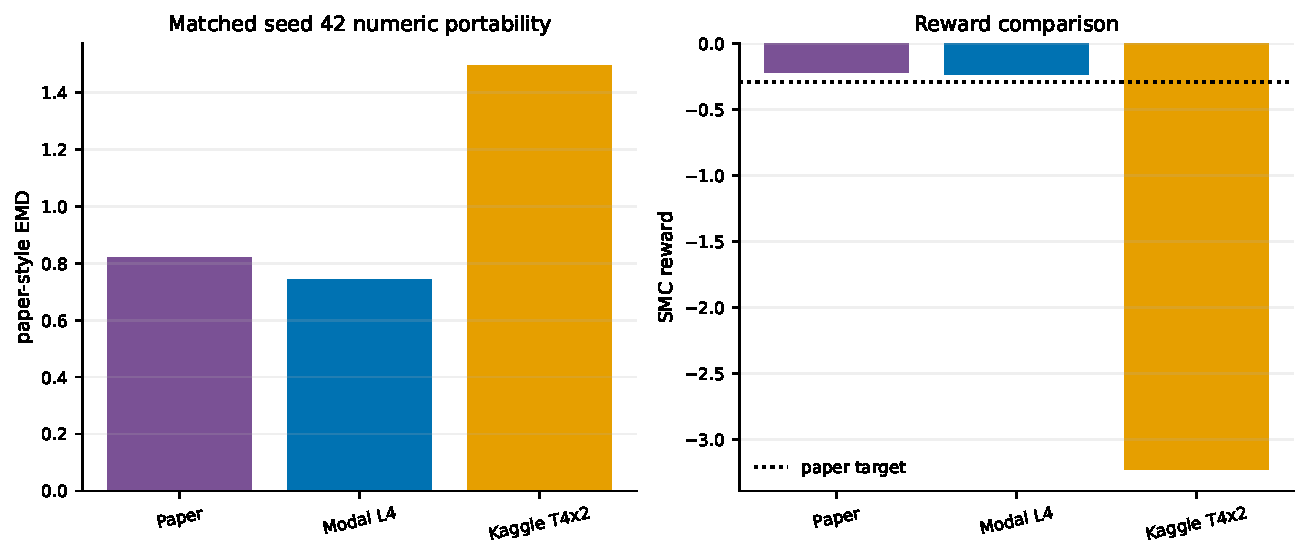
\includegraphics[width=0.88\textwidth]{figures/fig_das_kaggle_rescue.pdf}
\caption{Matched seed 42 trên hai backend. Cùng source/seed không đảm bảo bitwise equivalence giữa GPU architecture.}
\label{fig:kaggle}
\end{figure}

Verdict được tách:
\begin{itemize}
  \item \textbf{Infrastructure/execution: \PASS.} Hai T4 được xác nhận và payload seed 42/Numba 42 hoàn chỉnh.
  \item \textbf{Paper numeric match: \textbf{\KagglePaperVerdict}.} EMD \KaggleEMD{}, sai khác \KagglePaperSymDiff{} so với 0.82.
  \item \textbf{Cross-backend portability: \textbf{\KaggleModalVerdict}.} Sai khác đối xứng Kaggle--Modal là \KaggleModalSymDiff{}.
\end{itemize}

\section{FK Steering và Feynman--Kac Correctors}

\subsection{FK Steering}

Phạm vi là prompt ``a photo of a brown knife and a blue donut'', seed 42--44, $k=4$, 100 inference steps, $\lambda=2$, ImageReward; so sánh FK-max, FK-difference và base. Repo model cũ \nolinkurl{stabilityai/stable-diffusion-2-1} trả 401 nên runtime dùng public mirror \nolinkurl{sd2-community/stable-diffusion-2-1}; artifact identity drift này ngăn exact benchmark claim.

\begin{figure}[H]
\centering
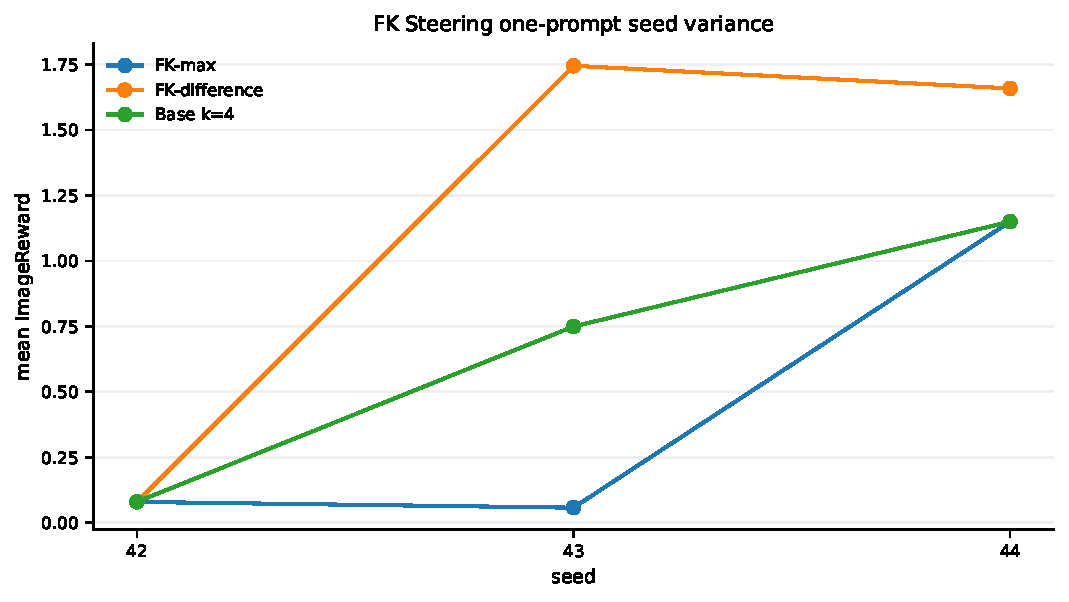
\includegraphics[width=0.72\textwidth]{figures/fig_fk_steering_variance_final.pdf}
\caption{One-prompt ImageReward thay đổi mạnh theo seed và thay đổi ranking. Kết quả đủ cho pipeline reproduction, không đủ cho GenEval superiority.}
\end{figure}

FK-difference đạt mean 1.161 với SD 0.938; base đạt 0.660 với SD 0.541. Với một prompt và ba seed, verdict là \PARTIAL.

\subsection{Feynman--Kac Correctors}

Paper Table~A1 dùng 10,000 samples, 1000 integration steps và 5 runs. Reproduction chạy đúng cấu hình này cho target-score và tempered-noise, mỗi proposal gồm no-FKC, birth--death clock (BDC) và systematic FKC. Notebook upstream có mismatch ở lời gọi BDC: caller khởi tạo accumulator một chiều với \code{reset\_transition\_per\_index=False} nhưng không truyền cờ vào sampler, khiến sampler dùng default \code{True} dành cho accumulator hai chiều. Runtime copy chỉ forward đúng cờ đã có; manifest lưu source/runtime/executed hashes và upstream clone vẫn sạch.

\begin{table}[H]
\centering
\small
\caption{Table~A1 paper và reproduction, đều là mean $\pm$ sample SD qua năm run. Tất cả metric lower-is-better.}
\begin{tabular}{@{}p{3.15cm}lrrrrr@{}}
\toprule
Method & Source & Energy-W2 & MMD & TV & W1 & W2 \\
\midrule
Target score / no FKC & Paper & 0.943$\pm$0.026 & 0.020$\pm$0.001 & 0.487$\pm$0.007 & 11.304$\pm$0.296 & 15.671$\pm$0.269 \\
 & Repro & 0.935$\pm$0.008 & 0.021$\pm$0.000 & 0.488$\pm$0.001 & 11.467$\pm$0.182 & 15.869$\pm$0.225 \\ \addlinespace[1.5pt]
Tempered noise / no FKC & Paper & 1.032$\pm$0.012 & 0.058$\pm$0.001 & 0.638$\pm$0.002 & 16.051$\pm$0.123 & 19.627$\pm$0.101 \\
 & Repro & 1.036$\pm$0.011 & 0.059$\pm$0.002 & 0.635$\pm$0.006 & 15.916$\pm$0.174 & 19.505$\pm$0.160 \\ \addlinespace[1.5pt]
Target score / BDC & Paper & 1.064$\pm$0.369 & 0.010$\pm$0.004 & 0.402$\pm$0.029 & 7.797$\pm$3.990 & 12.451$\pm$5.417 \\
 & Repro & 1.211$\pm$0.300 & 0.005$\pm$0.003 & 0.355$\pm$0.014 & 5.397$\pm$3.407 & 9.547$\pm$4.800 \\ \addlinespace[1.5pt]
Tempered noise / BDC & Paper & 1.228$\pm$0.401 & 0.056$\pm$0.029 & 0.572$\pm$0.055 & 12.598$\pm$4.155 & 17.679$\pm$4.178 \\
 & Repro & 1.108$\pm$0.294 & 0.054$\pm$0.068 & 0.546$\pm$0.082 & 12.030$\pm$7.061 & 16.037$\pm$7.819 \\ \addlinespace[1.5pt]
Target score / systematic & Paper & 1.098$\pm$0.418 & 0.007$\pm$0.005 & 0.372$\pm$0.020 & 6.256$\pm$3.960 & 11.265$\pm$5.629 \\
 & Repro & 0.891$\pm$0.105 & 0.007$\pm$0.004 & 0.382$\pm$0.031 & 8.221$\pm$6.017 & 13.727$\pm$7.202 \\ \addlinespace[1.5pt]
Tempered noise / systematic & Paper & 0.926$\pm$0.248 & 0.027$\pm$0.011 & 0.512$\pm$0.017 & 9.974$\pm$1.229 & 14.045$\pm$1.308 \\
 & Repro & 0.835$\pm$0.195 & 0.035$\pm$0.023 & 0.527$\pm$0.045 & 10.993$\pm$3.364 & 15.057$\pm$3.502 \\ \addlinespace[1.5pt]
\bottomrule

\end{tabular}
\end{table}

\begin{figure}[H]
\centering
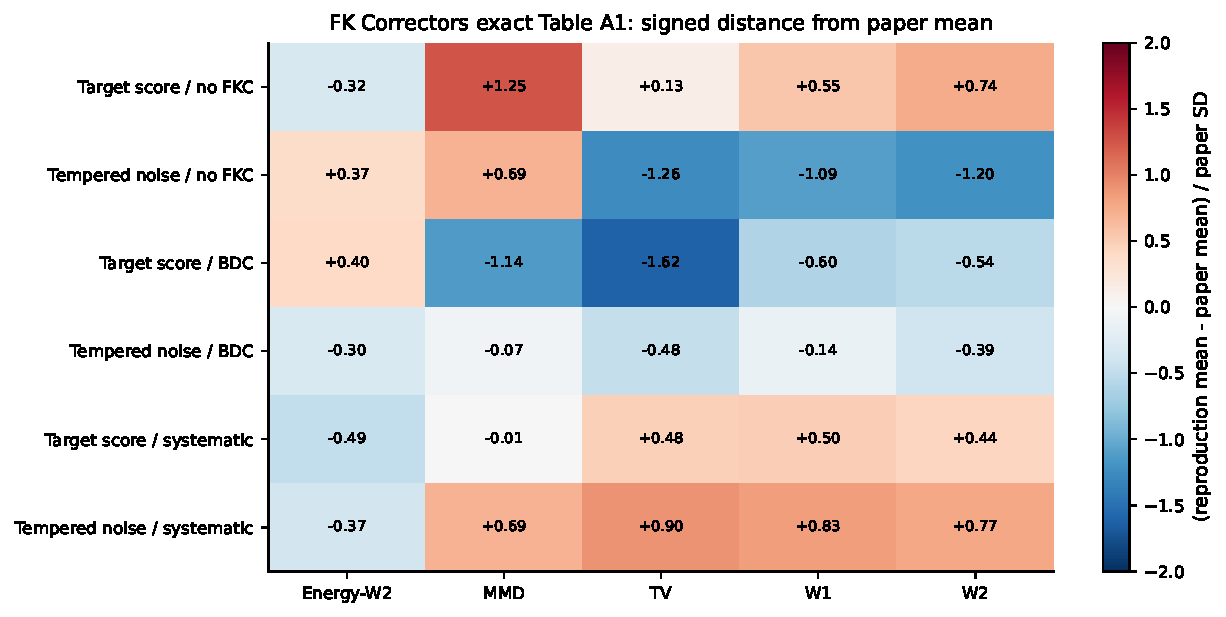
\includegraphics[width=0.88\textwidth]{figures/fig_fkc_relative_error_final.pdf}
\caption{Signed cell distance $(\bar{x}_{\mathrm{repro}}-\bar{x}_{\mathrm{paper}})/s_{\mathrm{paper}}$. Cả 30 ô nằm giữa $-2$ và $+2$; \FKCWithinOneSD/30 nằm trong $\pm1$ SD.}
\end{figure}

\begin{figure}[H]
\centering
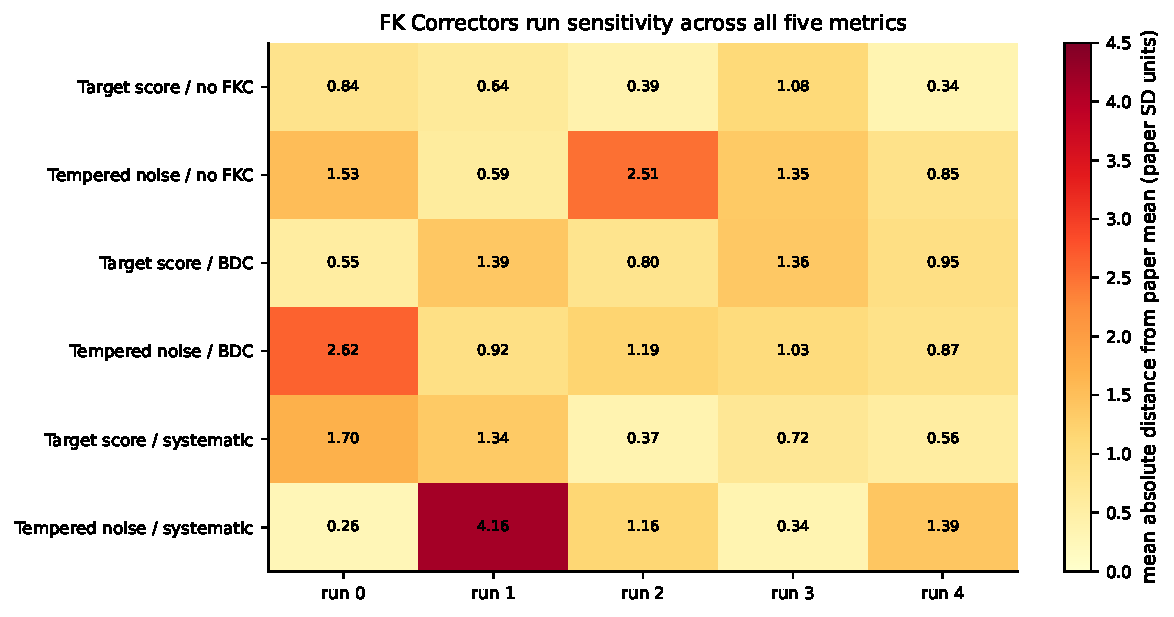
\includegraphics[width=0.88\textwidth]{figures/fig_fkc_run_variance_final.pdf}
\caption{Sensitivity của từng sequential run, tổng hợp năm metric bằng mean absolute distance theo paper SD. Upstream đặt tên loop variable là \code{seed} nhưng không reseed, nên hình không gán seed ID giả.}
\end{figure}

Kết quả exact đạt \FKCWithinTwoSD/30 ô trong $\pm2$ paper SD và \FKCWithinOneSD/30 ô trong $\pm1$ SD. Hướng corrected-minus-no-FKC đồng thuận \FKCDirectionAgreement/20 so sánh. Ngoại lệ duy nhất là target-score systematic Energy-W2: paper mean tăng 0.155 (xấu hơn) nhưng reproduction mean giảm 0.043; cả hai có SD lớn và overlap mạnh nên không đủ bằng chứng cho một direction claim. Variance run không nhỏ: tempered-noise BDC run~0 có W2 29.925 và MMD 0.176, còn bốn run kia có W2 11.108--13.646 và MMD 0.020--0.029. Tempered-noise systematic run~1 cũng là run xấu rõ rệt (W2 20.849, MMD 0.075). Vì vậy verdict là \PWV: exact protocol và numeric compatibility pass, nhưng không được che instability bằng mean.

\section{Chi phí, portability và tính toàn vẹn}

Ba Modal profile đều áp monthly budget 30 USD, reserve 1 USD và hard stop 29 USD. Mỗi submission được chặn nếu provider-reported usage cộng estimate vượt 29 USD; reserve đã được mã hóa trực tiếp bằng hard limit thấp hơn budget 1 USD nên guard không cộng hai lần. Seed 42--43 được chia thành tám shard L40S trên mỗi profile. Seed~44 ban đầu chia tám shard L4; sau snapshot 23:00 UTC và extrapolation conservative, shard [7,14) được dừng. Bốn prompt đã commit được cứu bằng hash và remote post-scoring; chỉ ba prompt chưa hoàn tất mới chạy lại trên L40S. Với FK Correctors, canary BDC pass trước full run; full bị profile thứ nhất chặn spend-limit trước submit, profile thứ hai chặn do runner chung khai báo L40S không liên quan, rồi runner L4 độc lập hoàn tất trên \code{phamvanvuhoan}. Hai lỗi pre-workload không được tính là scientific failures. Billing provider có thể trễ, nên snapshot cuối từ provider và ledger được lưu cùng report artifact thay vì suy ngược chi phí từ wall time.

\begin{table}[H]
\centering
\small
\caption{Snapshot cuối do Modal CLI báo, USD. Canonical cost được join theo đúng 26 scientific app ID đứng sau 25 artifact record; cả usage và cost đều có thể chịu billing lag.}
\begin{tabular}{@{}lrrr@{}}
\toprule
Profile & Final reported usage & Canonical app cost & Headroom tới 29 \\
\midrule
kieusontung6 & \BillingTungSixUsage{} & \BillingTungSixCost{} & \BillingTungSixHeadroom{} \\
kieusontung8 & \BillingTungEightUsage{} & \BillingTungEightCost{} & \BillingTungEightHeadroom{} \\
phamvanvuhoan & \BillingVuHoanUsage{} & \BillingVuHoanCost{} & \BillingVuHoanHeadroom{} \\
\bottomrule
\end{tabular}
\end{table}

Talapas không được dùng cho scientific payload vì phiên làm việc này không có ControlMaster/Duo hợp lệ. Báo cáo không biến việc không thể đăng nhập remote thành experimental failure.

\section{Threats to validity}

\begin{itemize}
  \item \textbf{Null-TTA seed identity:} paper chỉ nói ba random seed; $\{42,43,44\}$ là lựa chọn protocol, không chứng minh trùng seed tác giả.
  \item \textbf{Null-TTA mixed hardware:} seed 42--43 chạy L40S; seed 44 có bảy artifact L4, một prefix sinh trên L4/post-score trên L40S và một artifact L40S. Tất cả seed~44 dùng scorer tuần tự. Hardware-dependent floating-point drift có thể góp vào within/between-seed variance.
  \item \textbf{Null-TTA secondary scorers trên L4:} PickScore primary của seed~44 được tính trực tiếp trong official generation path. Ba secondary scorer được chạy lại từ PNG 8-bit do example chính thức lưu; PNG encoding là lossless đối với mảng đã quantize, nhưng bước tensor-to-uint8 trước đó có thể tạo lệch nhỏ so với chấm trực tiếp tensor. Vì vậy secondary-match phải đọc với caveat này.
  \item \textbf{Null-TTA scope:} chỉ Table~1 SD-v1.5/PickScore-target, chưa bao phủ SDXL, other reward targets hoặc mọi ablation.
  \item \textbf{DAS scope:} chỉ toy GMM Figure~1, không phải text-to-image experiments.
  \item \textbf{DAS estimator:} paper cho một EMD point từ subsample 500; 100-repeat estimator của report đo estimator noise nhưng không phải metric paper mới.
  \item \textbf{DAS seed criterion:} seed 42 là canonical vì code default; việc seed Numba bằng 42 là rescue hợp lý nhưng upstream không công bố Numba state đã dùng để tạo figure.
  \item \textbf{Kaggle utilization:} allocation có hai T4, scientific notebook dùng một GPU. Không có claim scaling/speedup.
  \item \textbf{FK Steering scope:} chỉ một prompt và model mirror, không đại diện GenEval.
  \item \textbf{FK Correctors run identity:} upstream loop variable tên \code{seed} nhưng không gọi reseed và tái sử dụng cùng initial prior sample tensor; năm hàng là sequential stochastic runs đúng code, không phải năm seed ID độc lập đã biết.
  \item \textbf{FK Correctors runtime repair:} BDC cần forward cờ shape mode tại một call site. Đây là sửa mismatch có bằng chứng tĩnh và canary, nhưng môi trường bitwise mà tác giả dùng để tạo table không được công bố; report không gọi bản vá là upstream-author-confirmed.
  \item \textbf{FK compatibility rule:} paper mean $\pm2$ SD là descriptive band, không phải CI hoặc test equivalence. PASS nghĩa là exact protocol và cell compatibility, không chứng minh hai data-generating processes đồng nhất.
\end{itemize}

\section{Kết luận}

Null-TTA được đánh giá bằng ma trận đầy đủ 3 seed $\times$ 50 prompt và bốn scorer, không bằng một canary đẹp. DAS được cứu bằng cách khóa RNG Numba bị bỏ sót: canonical seed 42 tái lập sát paper, trong khi seed 43 chứng minh variance là failure mode thực. Kaggle r6 tách đúng infrastructure success khỏi numeric match. FK Correctors nay không còn là scaled subset: full exact Table~A1 đạt 30/30 cell compatibility nhưng các run xấu BDC/systematic cho thấy vì sao mean phải đi kèm variance. Cách báo cáo này đáp ứng yêu cầu quan trọng nhất: nếu target là 0.29 và prior là 0.22, một số 0.21 không được gọi là thắng chỉ vì nhìn ``cao'' hay ``thấp'' hơn; metric, hướng tối ưu, baseline và variance phải được định nghĩa trước.

\section*{Data availability và lệnh tái lập}

Artifact machine-readable nằm trong \nolinkurl{results/*.json}; raw executed notebooks, metrics, NPZ, logs và accelerator evidence nằm trong \nolinkurl{remote_artifacts/} và \nolinkurl{outputs/kaggle_jobs/}. Figure/table trace lưu SHA-256 của mọi input được report dùng. Entrypoint remote là \nolinkurl{scripts/modal_null_tta.py}, \nolinkurl{scripts/modal_runner.py}, runner FK Correctors L4-only \nolinkurl{scripts/modal_fkc_table_a1.py} và source Kaggle \nolinkurl{kaggle/das_seed42.py}. Không có secret/token trong report package.

\section*{AI Disclosure}

This report was prepared with AI assistance for source auditing, remote experiment orchestration, statistical aggregation, visualization, and formatting. The user specified the scope and acceptance constraints. Numerical claims are gated by archived machine-readable artifacts; the report owner remains responsible for external use.

\appendix
\section{Engineering retries không được tính là scientific failures}

Kaggle attempts trước r6 đều terminal trước khi sinh \code{das\_metrics.json}: r2 instrument notebook hai lần; r3/r4 không tìm được repo dataset vì backend không mount source thứ hai; r5 embed source thành công và xác nhận T4x2 nhưng thiếu \code{CUBLAS\_WORKSPACE\_CONFIG} trước khi child kernel khởi tạo. r6 sửa đúng biến môi trường đó và mới được phép đưa vào bảng khoa học. Giữ log các retry giúp audit nguyên nhân; số lượng retry không được đổi thành ``hai lần model fail''.

Các DAS Modal năm-seed cũ cũng bị loại khỏi primary analysis vì chỉ seed NumPy/Python/Torch, không seed RNG Numba. Chúng là forensic evidence cho root cause, không phải dữ liệu để cộng vào matched-RNG aggregate. Với Null-TTA, L4 canary $n_{\max}=5$ chỉ dùng đo VRAM/throughput; canceled L40S fragments seed~44 không được trộn với full $n_{\max}=55$ matrix. Riêng L4 shard [7,14) đã chạy đúng $n_{\max}=55$ và commit bốn hàng hoàn chỉnh [7,11) trước khi dừng: CSV cùng tám PNG được kiểm SHA-256, bốn prompt này được remote post-score và nhận; suffix chưa hoàn tất [11,14) bị loại và chạy mới. Retry L40S trên workspace thứ hai dừng với \code{ConflictError: workspace ... is disabled}; đây là provider failure, không phải model failure, và không có row nào từ retry đó đi vào aggregate.

FK Correctors BDC canary lần đầu hoàn tất sampling nhưng dừng ở plotting-only cell vì canary bỏ baseline tạo biến \code{log\_weights\_scaled}; run này không sinh Table~A1 metric và được giữ như engineering failure. Canary lần hai bỏ đúng hai auxiliary plotting cells, hoàn tất hai BDC methods $\times$ hai runs. Full attempt trên \code{kieusontung8} bị provider spend-limit chặn trước app creation; attempt tiếp theo trên \code{phamvanvuhoan} bị Modal validate một hàm Null-TTA L40S không liên quan trong runner chung. Runner L4-only tách riêng giải quyết coupling cấu hình và full r3 mới là scientific artifact duy nhất đi vào Table~A1 aggregate.

\section{Checklist build}

\begin{itemize}
  \item[$\checkmark$] Null-TTA aggregator yêu cầu đúng 150 seed--prompt records và bốn scorer thật.
  \item[$\checkmark$] DAS aggregator yêu cầu matched seed và 3/3 mode coverage ở mọi run.
  \item[$\checkmark$] Kaggle report gate yêu cầu payload PASS, seed/Numba 42 và đúng hai GPU T4.
  \item[$\checkmark$] FK Correctors gate yêu cầu đúng 10k/1000/5, đủ 6 methods, 30 raw run rows và 30/30 cell compatibility.
  \item[$\checkmark$] Runtime patch manifest lưu hash source/runtime/executed notebook; upstream FK Correctors clone phải sạch.
  \item[$\checkmark$] Mọi figure/table sinh từ JSON/NPZ; không chép tay result remote.
  \item[$\checkmark$] PDF phải qua text preflight và render kiểm tra toàn bộ trang trước khi phát hành.
\end{itemize}

\bibliographystyle{plainnat}
\bibliography{references}

\end{document}
